% TO DO: add citations in thesis work, better research plan

\documentclass[10pt]{beamer}
\usetheme[height=0mm]{Rochester}
\usefonttheme[onlylarge]{structurebold}
\setbeamerfont*{frametitle}{size=\normalsize,series=\bfseries}
\setbeamertemplate{navigation symbols}{}
\setbeamercovered{dynamic}
\setbeamertemplate{itemize item}[triangle]
\setbeamertemplate{itemize subitem}[triangle]
%\useoutertheme{infolines}

%  use Darmstadt if commenting the next line
\usepackage[footheight=1em]{beamerthemeboxes}
\usepackage[natbib=true,backend=biber,citestyle=authoryear]{biblatex}
\bibliography{stats,../bib/stats,../bib/learning}

\usepackage{amsmath,amssymb,amsthm,bbm}             % AMS Math
\usepackage[utf8]{inputenc}
\usepackage[english]{babel}
\usepackage{myAlgorithm}
\usepackage{xcolor}
\usepackage{graphicx}
\usepackage{subfigure}
\usepackage{hyperref}
\usepackage{mathtools}
\usepackage{mathrsfs}
\usepackage{wasysym}
\usepackage{tikz}
\usetikzlibrary{bayesnet}
\usetikzlibrary{arrows}
\usepackage{url}

% notation
\DeclareMathOperator*{\argmax}{arg\,max}
\DeclareMathOperator*{\argmin}{arg\,min}
\newcommand{\cA}{\mathcal{A}}
\newcommand{\cS}{\mathcal{S}}
\newcommand{\cF}{\mathcal{F}}
\newcommand{\cX}{\mathcal{X}}
\newcommand{\cY}{\mathcal{Y}}
\newcommand{\cZ}{\mathcal{Z}}
\newcommand{\cN}{\mathcal{N}}
\newcommand{\cO}{\mathcal{O}}
\renewcommand{\leq}{\leqslant}
\renewcommand{\geq}{\geqslant}
\renewcommand{\phi}{\varphi}
\renewcommand{\epsilon}{\varepsilon}
\renewcommand{\d}{ {\rm d}}
\renewcommand{\emptyset}{\varnothing}

\newcommand\un[1]{\textcolor{magenta}{#1}}
\newcommand\unn[1]{\textcolor{blue}{#1}}
\newcommand\unnn[1]{\textcolor{red}{#1}}
\newcommand\unnnn[1]{\textcolor{orange}{#1}}

\def\cX{\mathcal{X}}
\def\cY{\mathcal{Y}}
\def\cZ{\mathcal{Z}}
\def\cS{\mathcal{S}}
\def\cR{\mathcal{R}}
\def\cA{\mathcal{A}}

\def\by{\mathbf{y}}

% indicator
\newcommand\IND[1]{\mathbbm{1}_{\{#1\}}}

\def\cfdemo{\url{https://chi-feng.github.io/mcmc-demo/}}

\def\tpi{\widetilde{\pi}}
\def\cN{\mathcal{N}}
\renewcommand\d{\mathrm{d}}
\def\e{\mathrm{e}}

\usecolortheme[named=bleu]{structure}

\title[Bayesian ML: what, why, and how?]{Bayesian ML: what, why, and how?}
%\subtitle{\url{http://github.com/rbardenet/bml-course}}
\author[Rémi Bardenet (CNRS \& Univ. Lille)] % (optional, for multiple authors)
{Rémi Bardenet}
\institute[] % (optional)
{
  CNRS \& CRIStAL, Univ. Lille, France\\
\vspace{1cm}

\includegraphics[width=0.15\textwidth]{Logos/logo_CNRS.pdf}
\qquad \includegraphics[width=0.35\textwidth]{Logos/logo_CRISTAL}
\qquad
\includegraphics[width=0.15\textwidth]{Logos/logo_ERC}
\qquad 
\includegraphics[width=0.13\textwidth]{Logos/logo_funded_by_ANR}
}
\date{}

\begin{document}
\begin{frame}
\maketitle
\end{frame}

\begin{frame}
\frametitle{Outline}
\tableofcontents
\end{frame}

%%%%%%%%%%%%%%%%%%%%%%
\section{Introduction}
%%%%%%%%%%%%%%%%%%%%%%


\section{Bayesian ML: what is it?}

\subsection{A few illustrative examples}

\begin{frame}
  \frametitle{Regression as a decision problem}
\end{frame}

\begin{frame}
  \frametitle{Classification as a decision problem}
\end{frame}

% \begin{frame}
%   \frametitle{A quick motivating example before we go formal 1/2}
%   \begin{itemize}
%     \vfill\item Let $N$ individuals evolve from Susceptible to Infected to Recovered, $x_n(t) \in\{S,I,R\}$, $1\leq n\leq N$, $t\in[0,T]$.
%     \vfill\item Each susceptible individual $n$ moves to $R$ according to a Poisson process with intensity
%     $$\sum_{k:x_k(t)=I} \lambda_{nk}(\unn{\theta_{SI}}).$$
%     \vfill\item Each infected person recovers after a Gamma(\unn{$a,b$}) time.
%     \vfill\item This allows to express
%     $$
%     p(x_1(t_{1,1}), \dots, x_1(t_{1,T_1}), \cdots, x_n(t_{n,1}), \dots, x_1(t_{n,T_n})\vert \unn{\theta}).
%     $$
%     where \unn{$\theta= (\theta_{SI}, a, b)$}.
%     \vfill\item Now, consider $p(\theta\vert \text{data}) \propto p(\text{data}\vert \theta) \un{p(\theta)}.$
%   \end{itemize}
% \end{frame}

% \begin{frame}
% \frametitle{A quick motivating example before we go formal 2/2}
%   \begin{itemize}
%   \vfill\item If asked to report an interval on a particular function of $\theta$, say $R_0$, I would output a small interval $I$ such that
%   $$ \int_I p(\theta\vert \text{data}) \,\d\theta \geq 0.95.$$
%   \vfill\item If asked whether we should close universities, I would ask for
%   \begin{itemize}
%     \item \un{the cost $\alpha$ of closing unis when $R_0<1$},
%     \item \unn{the cost $\beta$ of keeping unis open while $R_0>1$}.
%   \end{itemize}
%   \vfill\item Then I would recommend closing if and only if
%   $$
%   p(R_0>1\vert \text{data}) > \frac{\un{\alpha}}{\un{\alpha}+\unn{\beta}}.
%   $$
%   \vfill\item Additionally, I would check that the decision doesn't change if I change my prior $p(\theta)$ a little.
%   \vfill\item If it did, then I would refine my likelihood and/or wait for more data.
% \end{itemize}

% \tikz{ %
  %   \node[latent] (S) {$S$};%
  %   \node[latent,right=of S] (I) {$I$}; %
  %   \node[latent,right=of I] (R) {$R$}; %
  %   \edge S I;
  %   \edge I R;
  % }
% \end{frame}

% \begin{frame}{Quotes from \citep{GCSDVR13} on Bayesian methods}
% % put book picture
% \begin{itemize}
%  \vfill\item \emph{[...] practical methods for making inferences from data, using probability models for quantities we observe \un{and for quantities about which we wish to learn}.}
% \vfill\item \emph{The essential characteristic of Bayesian methods is their \un{explicit use of probability for quantifying uncertainty} in inferences based on statistical data analysis.}
% \vfill\item \emph{Three steps:
% \begin{enumerate}
%   \item Setting up a full probability model,
%   \item Conditioning on observed data, calculating and interpreting the appropriate ``posterior distribution",
%   \item Evaluating the fit of the model and the implications of the resulting posterior distribution. In response, one can alter or expand the model and repeat the three steps.
% \end{enumerate}
% }
% \end{itemize}
% \end{frame}

% \begin{frame}{Notation that I will try to stick to}
% \begin{itemize}
%   \vfill\item $y_{1:n} = (y_1,\dots,y_n) \in \cY^n$ denote observable data/labels.
%   \vfill\item $x_{1:n} \in \cX^n$ denote covariates/features/hidden states.
%   \vfill\item $z_{1:n} \in \cZ^n$ denote hidden variables.
%   \vfill\item $\theta\in\Theta$ denote parameters.
%   \vfill\item $X$ denotes an $\cX$-valued random variable. Lowercase $x$ denotes either a point in $\cX$ or an $\cX$-valued random variable.
% \end{itemize}
% \end{frame}

% \begin{frame}{More notation}
%   \begin{itemize}
%   \vfill\item Whenever it can easily be made formal,
%   %(by choosing an appropriate reference $\sigma$-finite measure, say Lebesgue or the counting measure),
%   we write densities for our random variables and let the context indicate what is meant. So if $X\sim \cN(0,\sigma^2)$, we write
%   $$ \mathbb E h(X) = \int h(x) \frac{e^{-x^2/2\sigma^2}}{\sigma\sqrt{2\pi}}\d x = \int h(x)p(x)\mathrm{d}x.$$
%   Similarly, for $X\sim \mathcal P(\lambda)$, we write
%   $$ \mathbb E h(X) = \sum_{k=0}^\infty h(k) e^{-\lambda}\frac{\lambda^k}{k!} = \int h(x) p(x)\mathrm{d} x$$
%   \vfill\item All pdfs are denoted by $p$, so that, e. g.
%   \begin{align*}
% \mathbb{E} h(Y, \theta) &= \int h(y, \theta)p(y, \theta)\,\d y\d \theta\\
% &= \int h(y, \theta)p(y, x, \theta) \,\d x\d y \d\theta\\
% &= \int h(y, \theta) p(y, \theta\vert x)p(x) \,\d x\d y \d\theta
%   \end{align*}
% \end{itemize}

% \end{frame}

\subsection{ML as data-driven decision-making}
\begin{frame}{Abraham Wald (1902--1950)}
  \centering
  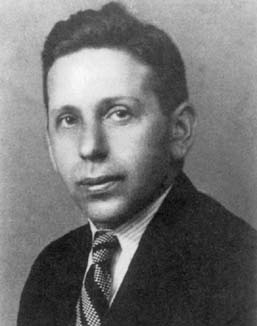
\includegraphics[width=\twofig]{\figdir/wald.jpg}
\end{frame}

\begin{frame}{Describing a decision problem under uncertainty}
\begin{itemize}
  \vfill\item A state space $\cS$,\\
  \un{Every quantity you need to consider to make your decision.}
  \vfill\item Actions $\cA \subset \cF(\cS, \cZ)$,\\
  \un{Making a decision means picking one of the available actions.}
  \vfill\item A reward space $\cZ$,\\
  \un{Encodes how you feel about having picked a particular action.}
  \vfill\item A loss function $L:\cA\times \cS \rightarrow \mathbb{R}_+$.\\
  \un{How much you would suffer from picking action $a$ in state $s$. It is also customary to first define a utility $u:\cZ\rightarrow \mathbb{R}_+$, and then let
  $$ L(a,s) = \sup_{a'\in\cA} u\big(a'(s)\big) - u\big(a(s)\big) \in\mathbb{R}_+.$$
  }
\end{itemize}
\end{frame}

\begin{frame}{Classification as a decision problem}
\begin{itemize}
\item $\cS = \un{\cX^n\times\cY^n}\times \cX\times \cY$, i.e. $s = (x_{1:n}, y_{1:n}, x, y)$.
\item $\cZ = \{0,1\}$.
\item $\cA = \{a_g: s\mapsto 1_{y\neq g(x; \un{x_{1:n}, y_{1:n}})}, \quad g\in\mathcal{G}\}$.
\item $L(a_g,s) = 1_{y\neq g(x; \un{x_{1:n}, y_{1:n}})}$.
\end{itemize}
\vfill
\begin{block}{PAC bounds; see e.g. \citep{ShBe14}}
Let $(x_{1:n},y_{1:n})\sim \mathbb{P}^{\otimes n}$, and independently $(x,y)\sim \mathbb{P}$, we want an algorithm $g(\cdot; x_{1:n}, y_{1:n})\in\mathcal G$ such that if $n\geq n(\delta,\epsilon)$,
$$
\un{\mathbb{P}^{\otimes n}}\left[\mathbb{E}_{(x,y)\sim \mathbb P} L(a_g,s) \leq \epsilon\right] \geq 1-\delta.
$$
\end{block}\end{frame}

\begin{frame}{Regression as a decision problem}
  \begin{itemize}
  \item $\cS = $
  \item $\cZ = $
  \item $\cA = $
  \item
  \end{itemize}
  \blank
\end{frame}

\begin{frame}{Estimation as a decision problem}
  \begin{itemize}
  \item $\cS = $
  \item $\cZ = $
  \item $\cA = $
  \item
  \end{itemize}
  \blank
\end{frame}

\begin{frame}{Topic modeling as a decision problem}
  \begin{itemize}
    \item $\cS = $
    \item $\cZ = $
    \item $\cA = $
    \item
    \end{itemize}
    \blank
  \end{frame}

  \begin{frame}{Model choice as a decision problem}
    \begin{itemize}
      \item $\cS = $
      \item $\cZ = $
      \item $\cA = $
      \item
      \end{itemize}
      \blank
    \end{frame}
  

% Regression, classification, estimation, dimensionality reduction, clustering, topic modelling as a more complex hidden variable model: gives states and losses, maybe state the main non-Bayesian solution.

\subsection{Subjective expected utility}
% State the principle, insist on the choice of p, comment on BDA.
% Recap on graphical models
% List all previous examples and show a graphical model and the Bayes action.
% Solve a few examples, link with non-Bayesian solutions like regularized regression. Horseshoe?
% Confront with preconceived ideas on BML. Insist that on top of being a general, interpretable principle, SEU is usually good for non-Bayesians too: BvM, smaller MSE, PAC-Bayes (to come). Moreover, philosophical support (also to come in lecture on foundations).
\begin{frame}{SEU is what defines the Bayesian approach}
\begin{block}{The subjective expected utility principle}
\begin{enumerate}
\item \un{Choose} $\cS, \cZ, \cA$ and a loss function $L(a,s)$,
\item \un{Choose} a distribution $p$ over $\cS$,
\item Take the the corresponding \un{Bayes action}
\begin{equation}
a^\star \in \argmin_{a\in\mathcal{A}} \mathbb{E}_{s\sim p} L(a,s).
\label{e:seu}
\end{equation}
\end{enumerate}
\end{block}
\vfill

\begin{block}{Corollary: minimize the posterior expected loss}
If we partition $s=(s_{o}, s_{\text{u}})$, then
$$ a^\star \in \argmin_{a\in\mathcal{A}} \mathbb{E}_{s_{o}} \mathbb{E}_{s_{\text{u}}\vert s_{o}} L(a,s).$$
Equivalently to \eqref{e:seu}, given $s_o$, we choose
$$
a^\star = \delta(s_o) = \argmin_{a\in\mathcal{A}} \un{\mathbb{E}_{s_{\text{u}}\vert s_{o}} L(a,s)}.$$
\end{block}
\end{frame}

\subsection{Specifying joint models}
\begin{frame}{A recap on probabilistic graphical models}
  \begin{itemize}
    \item PGMs (aka ``Bayesian" networks) represent the dependencies in a joint distribution $p(y)$ by \un{a directed graph $G=(E,V)$}.
    \item Two important properties:
    $$
    p(y) = \prod_{v\in V} p(y\vert y_{\text{pa(v)}}) \qquad\text{and}\qquad
    y_v \perp y_{nd(v)} \vert y_{pa(v)}.
    $$
    \blank
    \item Also good to know how to determine whether $A\perp B\vert C$; see \citep[Section 10.5]{Mur12}.
  \end{itemize}
  \blank
\end{frame}

\begin{frame}{Estimation as a decision problem: point estimates}
\end{frame}

\begin{frame}{Estimation as a decision problem: credible intervals}
\end{frame}

\begin{frame}{Choosing priors (see Exercises)}
\end{frame}

\begin{frame}{Classification as a decision problem}
\end{frame}

\begin{frame}{Regression as a decision problem 1/2}
% Exercise: Gaussian-Gaussian model, smaller MSE as an example of having good frequentist properties
\end{frame}

\begin{frame}{Regression as a decision problem 2/2}
% Exercise: Gaussian-Gaussian model, smaller MSE as an example of having good frequentist properties
\end{frame}

\begin{frame}{Dimensionality reduction as a decision problem}
\end{frame}

\begin{frame}{Clustering as a decision problem}
\end{frame}

\begin{frame}{Topic modelling as a decision problem}
\end{frame}

\begin{frame}{Image denoising as a decision problem}
\begin{figure}
\includegraphics[width=\textwidth]{Figures/denoising.png}
\caption{Taken from \citep[Chapter 21]{Mur12}}
\end{figure}
\blank
\end{frame}

\subsection{50 shades of Bayes}
% prior should not depend on the data, then advisable to study the effect of the prior after the analysis is done.
% prior should be "non-informative", but then depends on data
% we prefer MAP so prior is only there to regularize -> mainly for computational convenience.
% Sometimes we can turn the ``Bayesianness knob". Example of sparse regression and the horseshoe prior.
\begin{frame}{50 shades of Bayes}
  \begin{alertblock}{An issue (or is it?)}
    Depending on how they interpret and how they implement SEU, you will meet many types of Bayesians (46656, according to Good).
  \end{alertblock}
\begin{block}{A few divisive questions}
\begin{itemize}
\item Using data or the likelihood to choose your prior; see Lecture \#5.
\item Using MAP estimators for their computational tractability, like in inverse problems
$$ \hat x_\lambda \in \argmin \Vert y- Ax\Vert + \lambda\Omega(x).$$
\item When and how should you revise your model (likelihood or prior)?
\item MCMC vs variational Bayes (more in Lectures \#2 and \#3)
\end{itemize}
\end{block}
\end{frame}

% ----------------------------------------------------------------------
\section{Bayesian ML: how do I implement it?}
% ----------------------------------------------------------------------
\begin{frame}{Expected utility requires computing integrals}
  \begin{block}{Minimizing the posterior expected loss}
  If we partition $s=(s_{o}, s_{\text{u}})$, then, given $s_o$, we choose
  $$
  a^\star = \delta(s_o) = \argmin_{a\in\mathcal{A}} \un{\mathbb{E}_{s_{\text{u}}\vert s_{o}} L(a,s)}.
  $$
\end{block}

  \begin{alertblock}{The bottleneck is computing integrals w.r.t. the posterior}
  \begin{itemize}
    \item E.g. for binary prediction with 0-1 loss
    $$
    y^\star \in \argmax_{y\in\{0,1\}} \int p(y\vert x,\theta) p(\theta\vert x_{1:n}, y_{1:n}) \d\theta
    $$
    \item or for estimation with squared loss
    $$
    \theta^\star = \int \theta p(\theta\vert y_{1:n}) \d\theta.
    $$
  \end{itemize}
\end{alertblock}
\end{frame}

\begin{frame}{Numerical integration}
  Let $\pi$ be a pdf w.r.t. $\d \theta$.

  \begin{block}{The problem of numerical integration}
    Find $T$ nodes
    $(\theta_t)$ and weights $(w_t)$ so that
    $$
    \int f(\theta)\pi(\theta)\d \theta \quad\approx\quad \sum_{t=1}^N w_t f(\theta_t), \quad \forall
    f\in\mathcal C,
    $$
    where $\mathcal C$ is a large class of functions.
  \end{block}
  \begin{alertblock}{A constraint for Bayesians: $\pi$ is only known up to a constant}
    E.g. in estimation,
    $$ \pi(\theta) = p(\theta\vert y_{1:n}) \propto p(y_{1:n}\vert\theta) p(\theta) =: \pi_u(\theta).$$
    Or in classification/regression,
    $$
    \pi(\theta) = p(\theta\vert x_{1:n}, y_{1:n}) \propto p(y_{1:n}\vert x_{1:n}, \theta) p(\theta)=: \pi_u(\theta).
    $$
  \end{alertblock}

  % \begin{exampleblock}{Main families of methods}
  %   \begin{itemize}
  %   \item variants of Riemann integration \cite{DaRa84},
  %   \item Gaussian quadrature \cite{Gau04},
  %   \item quasi-Monte Carlo methods \cite{DiKuSl13},
  %   \item \un{Monte Carlo methods \cite{RoCa04}: importance sampling, MCMC.}
  %   \end{itemize}
  % \end{exampleblock}
  \end{frame}

\begin{frame}{Riemann-like integration is impractical when $d\gg 1$.}
\blank
\begin{itemize}
\item For modern developments, see quasi-Monte Carlo integration \cite{DiPi10}.
\end{itemize}
\end{frame}

\subsection{Monte Carlo methods}
\begin{frame}{Monte Carlo integration}
\begin{block}{The Monte Carlo principle}
Find a distribution on $\theta_1,\dots,\theta_T$ and weights $w_t$ such that
$$ \un{\mathcal{E}_T(f) =  \sum_{t=1}^T w_t f(\theta_t) - \int f(\theta)\pi(\theta)\d \theta}$$
is small (with large probability, in quadratic mean, converges in law at some rate, etc.)
\end{block}
\begin{itemize}
  \item If you knew how to sample from $\pi$, you could take $\theta_t\sim\pi$ i.i.d., $w_t=1/T$, and prove e.g.
  $$ \mathbb{P}\left( \un{\mathcal{E}_T(f)} \geq \alpha\frac{\sigma(f)}{\sqrt{T}} \right) \leq \frac{1}{\alpha^2}, \quad \forall \alpha,$$
  as soon as $\sigma(f)^2 := \mathbb{V}_\pi [f(\theta) - \int f(\theta)\pi(\theta)\d\theta]<+\infty$.
\end{itemize}
\end{frame}

\begin{frame}{Self-normalized importance sampling}
\begin{itemize}
  \item Let $\pi_u(\theta) = Z\pi(\theta)$ be the unnormalized target pdf.
  \item Sample $\theta_{1:T}$ i.i.d. from $q$, and take
  $$
  w_t = \frac{\pi_u(\theta_t)}{q(\theta_t)} \times \left( \sum_{t=1}^T \frac{\pi_u(\theta_t)}{q(\theta_t)} \right)^{-1}
  $$
  so that $\sum w_t = 1$.
  \item Then
  $$$$
  \vfill
  \item One can show that $ \sqrt{T}\un{\mathcal{E}_T(f)} \rightarrow \cN(0, \sigma^2_{\text{NIS}}(f))$.
  \item Problem is that for reasonable choices of $f,q,\pi$, \un{$\log \sigma_{\text{NIS}}(f) \propto d$}.
\end{itemize}
\end{frame}

\subsection{The Metropolis-Hastings algorithm}

\begin{frame}{(Mostly) friendly faces}
\begin{figure}
  \hfill
  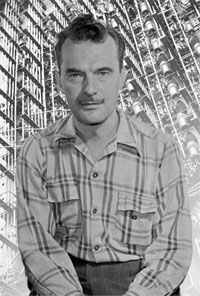
\includegraphics[width=\threefig]{Figures/metropolis}
  \hfill
  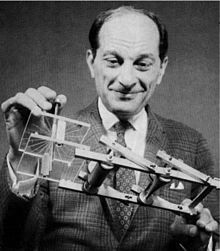
\includegraphics[width=\threefig]{Figures/ulam}
  \hfill
  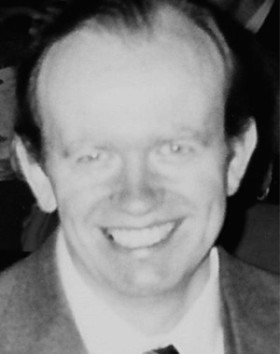
\includegraphics[width=\threefig]{Figures/hastings}
  \hfill
  \caption{A subset of MCMC pioneers: N. Metropolis, S. Ulam, W. K. Hastings}
\end{figure}\end{frame}

\begin{frame}{Markov chain Monte Carlo (MCMC; \citep{RoCa04})}
\begin{itemize}
  \item The idea is to take $(\theta_t)$ to be an ergodic Markov chain with limiting distribution $\pi$, so that for $f\in L^1(\pi)$,
  % $$
  % \lim \frac{1}{T} \sum_{t=1}^T f(\theta_t) \rightarrow \int f(\theta)\pi(\theta)\d\theta, a. s..
  % $$
  $$$$
  \vfill
  \item A Markov chain is specified by its kernel $P(\theta,\theta')$.
  \item We often try to prove that, with weak conditions on $\pi$ and $f$,
  % $$
  % \lim \sqrt{T}\mathcal E_T(f)  \rightarrow \cN(0,\sigma^2(f)),
  % $$
  $$$$
  \vfill
  and $\sigma^2(f)$ can be estimated; see \citep{DoMoSt14}.
  \item Most MCMC kernels are instances of the Metropolis-Hastings kernel.
  $$
  P_{\text{MH}}(\theta,\theta') = \unnnn{\alpha(\theta,\theta')} \un{q(\theta'\vert\theta)} + \delta_\theta(\theta')\left[1-\int \unnnn{\alpha(\theta,\vartheta)}\un{q(\vartheta\vert\theta)}\right]\d\vartheta,
  $$
  where
  $$
  \unnnn{\alpha(\theta,\theta')} = 1\wedge \frac{\pi(\theta')}{\pi(\theta)} \un{\frac{q(\theta\vert\theta')}{q(\theta'\vert\theta)}}.
  $$
  \end{itemize}
\end{frame}

\begin{frame}
\frametitle{The Metropolis-Hastings algorithm}
\begin{algorithm}{$\Algo{MH}\big(\unn{\pi_u},\, q(\cdot\vert\cdot),\,\theta_{0},\, T\big)$}
\Aitem \For $t\setto1$ \To $T$
\Aitem \mt $\theta\setto\theta_{t-1}$
\Aitem \mt $\theta'\sim \un{q(.\vert\theta)}$, $u\sim\mathcal U_{(0,1)}$,
\Aitem \mt $\rho =  \unn{\frac{\pi(\theta')}{\pi(\theta)}} \un{\frac{q(\theta\vert\theta')}{q(\theta'\vert\theta)}}$.
\Aitem \mt \If $u<\rho$,
\Aitem \mtt $\theta_{t}\setto\theta'$
\mt \algoremark{\unn{Accept}}
\Aitem \mt \Else $\theta_{t}\setto\theta$
\mt \algoremark{\unn{Reject}} \label{ai:acceptanceEnd}
\Aitem
\Return $(\theta_{t})_{t=1,\dots,N_{\text{iter}}}$
\end{algorithm}
\end{frame}

\begin{frame}{MH leaves $\pi$ invariant}
\begin{itemize}
  \item We first show detailed balance, i.e., $\pi(\theta)P(\theta,\theta') = \pi(\theta')P(\theta',\theta).$
  \vfill
  \vfill
  \vfill
  \vfill
  \item We deduce that $P$ leaves $\pi$ invariant.
  \vfill
  \vfill
  \vfill
  \vfill
  \item Note that if $P_1$ and $P_2$ leave $\pi$ invariant, then so does
  $$
  P_1P_2 (\theta,\theta') = \int P_1(\theta,\vartheta)P_2(\vartheta,\theta')\d\vartheta.
  $$
  \item The MH error scales polynomially with the dimension; see \href{P. Jacob's blog post}{https://statisfaction.wordpress.com/2018/05/15/scaling-of-mcmc-with-dimension-experiments/}

\end{itemize}
\end{frame}

\subsection{Gibbs sampling}
\begin{frame}{The random scan Gibbs sampler}
\begin{itemize}
\item Consider MH with
$$
\un{q(\theta'\vert\theta) = \frac1d \sum_{k=1}^d \pi(\theta_k\vert \theta_{\setminus k})}, \quad \theta_{\setminus k}:= (\theta_1,\dots,\theta_{k-1},\theta_{k+1},\dots,\theta_d).
$$
\item Then the probability of acceptance $\alpha(\theta,\theta')$ is always $1$.
$$$$
\vfill
\item In practice, the systematic scan Gibbs sampler is more common, which consists in repeatedly: drawing $\theta_1\vert\theta_{\setminus 1}$, then $\theta_2\vert\theta_{\setminus 2}$, etc. always conditioning on the newest values available of each $\theta_k$.
\item You can also partition $\theta$ in arbitrary blocks.
\end{itemize}
\end{frame}

\begin{frame}{An example: Latent Dirichlet allocation}

\end{frame}

\begin{frame}{Collapsed Gibbs sampling for LDA}

\end{frame}

\subsection{Hamiltonian Monte Carlo}
\begin{frame}{Hamiltonian dynamics is the source of inspiration}
\begin{block}{Hamilton's equations of motion}
Consider a physical system described by Hamiltonian $H(x,\xi)$ in phase space $(x,\xi)\in \mathbb{R}^{2d}$. Then the trajectories are prescribed by
\begin{equation}
  \label{e:hamilton}
  \dot{x_i} = \frac{\partial H}{\partial \xi_i} \qquad \dot{\xi_i} = -\frac{\partial H}{\partial x_i}.
\end{equation}
\end{block}
\begin{itemize}
  \item Given an initial point $(x,\xi)$, solve \eqref{e:hamilton} and denote the corresponding position in $\mathbb{R}^{2d}$ at time $t>0$ by $\Phi_t(x,\xi)$.
  \item \eqref{e:hamilton} implies that $t\mapsto H(\Phi_t(x,\xi))$ is constant.
  \item $\Phi_t$ has an inverse, and $\int_A \d x\d \xi = \int_{\Phi_t(A)} \d x\d \xi$.
  \item As an example, consider $H(x,\xi) = \frac12 x^2 + \frac12 \xi^2.$
\end{itemize}
\blank
% Describe, show Jacobian, show scaling with dimension, % discuss automatic differentiation and pymc3
\end{frame}

\begin{frame}{Hamiltonian Monte Carlo mimics a physical system}
  \begin{itemize}
    \item Let $\log \pi(x, \xi) =  \log \pi(x) + \frac12 \xi^T M(x) \xi$.
    \item For $t>0$ fixed, consider the Markov kernel $P((x,\xi), (x,\xi'))$ corresponding to
    $$ \xi\sim \cN(0,M(x)^{-1})$$
    followed  by
    $$(x',\xi') = \phi_T(x,\xi).$$
    Then $\pi(x,\xi)$ is invariant for $P$, and \un{so is its marginal $\pi(x)$}.
    \vspace{2.5cm}
    \item \un{Integrating the Hamilton flow can lead to long jumps} compared to MH with a Gaussian proposal, especially in high dimensions.
    \item In practice, $\phi_T$ has to be approximated, thus requiring an acceptance step. Paramaters like $T$ have to be tuned, as in NUT \citep{HoGe14}, which favors long jumps with no U-turns.
\end{itemize}
\end{frame}

% Show Chi Feng's demo.
\subsection{Convergence diagnostics for MCMC}
\begin{frame}{What can go wrong?}
\begin{figure}
\includegraphics[width=\textwidth]{Figures/cvDiagnostics}
\caption{Taken from \citep{GCSDVR13}}
\end{figure}
We need to monitor both cross-chain and within-chain behavior.
\end{frame}

\begin{frame}{Comparing $P$ chains with overdispersed starting points}
\begin{itemize}
  \item The behaviour of the $P$ traces should become similar.
  \item Always make visual sanity checks!
  \item Scalar estimates should converge to the same value.
  \item We can also compare the variance of a scalar estimate within- and across chains
\end{itemize}

  \begin{block}{The Gelman-Rubin diagnostic}
  \begin{itemize}
    \item Choose an $f$ of interest, e.g. $f(\theta) = \theta_1$.
    \item Compute $B:=\frac{T}{P-1}\sum_{p=1}^P (\bar f_{\cdot p} - \bar f_{\cdot\cdot})^2$.
    \item Compute $W:=\frac1P \sum_{p=1}^P\left[ \frac{1}{T-1} \sum_{t=1}^T (\bar f_{tp}-\bar f_{\cdot p})^2\right].$
    \item Then check whether
    $$\hat R = \sqrt{\frac{\un{\frac{T-1}{T}W + \frac1T B}}{\unnnn{W}}}\in[1,1.1].$$
  \end{itemize}
\end{block}
\end{frame}

\begin{frame}{More convergence diagnostics}
\begin{block}{Single-chain diagnostics}
  \begin{itemize}
  \item The idea is to compare different chunks of a single chain.
  \item At stationarity, large chunks should be statistically hard to distinguish.
  \item The \un{Geweke diagnostic} tests this similarity \citep{Gew04}
  \end{itemize}
\end{block}

\begin{block}{Effective sample size}
  \begin{itemize}
  \item Autocorrelation in each chain is what increases the variance of scalar estimands, compared to i.i.d. draws from $\pi$.
  \item We can estimate this autocorrelation, and build an estimator for the ratio of the two variances $\widehat{ESS}\in [1,PT]$, called the \un{\emph{effective sample size}}; see e.g. \citep[Section 11.5]{GCSDVR13}.
  \end{itemize}
\end{block}
\end{frame}


\begin{frame}{Conclusion}
\begin{block}{Take-home message}
  \begin{itemize}
    \item MCMC approximates the integrals in the expected utility framework.
    \item Try to \un{leverage the problem's structure} to design your kernels.
    \item Otherwise, try standard kernels like HMC.
    \item Always monitor convergence.
  \end{itemize}
\end{block}

\onslide<2>
  \begin{itemize}
  \item HMC with NUTS is the default choice in most probabilistic programming frameworks.
  \item MCMC is a \un{rich research topic}. Some keywords: Wang-Landau, Langevin, equi-energy, hit-and-run, bouncy particle sampler.
  \item Besides Markov chains, checkout \un{sequential Monte Carlo samplers} \citep{DeDoJa06}.
  \item Deterministic methods are also investigated: \un{quasi-Monte Carlo methods} \citep{DiPi10} have the best convergence rates as soon as the integrand is smooth.
\end{itemize}
\end{frame}


\subsection{Variational inference}
\begin{frame}{When MCMC is intractable, variational inference comes to help}
\begin{block}{Turning integration into optimization over measures}
Variational Bayesian inference (VB) consists in approximating
$$ \int f(\theta)\pi(\theta)\d\theta \approx \int f(\theta)q(\theta)\d\theta$$
with \un{$ q \in \argmin_{\tilde q\in \mathcal Q} \text{distance}(\pi, \tilde q)$}. Often we take
$$
\text{distance}(\pi, \tilde q) = \text{KL}(\tilde q, \pi) := \int q(\theta) \log \frac{q(\theta)}{\pi(\theta)}\d\theta.
$$
for computational convenience.
\end{block}
\blank
\end{frame}

\begin{frame}{But remember we can only evaluate $\pi_u = Z\pi$...}
\begin{itemize}
\item Show that $J(q) := \int q(\theta) \log \frac{q(\theta)}{\pi_u(\theta)}\d\theta = \text{KL}(q, \pi) - \log Z.$
\blank
\item In particular, $L(q) = -J(q) \leq \log Z$. For
$$
\pi_u(\theta) = p(\text{data}\vert\theta) p(\theta),
$$
$L(q)$ is thus \un{a lower bound for the evidence} $p(\text{data})$ (ELBO).
\end{itemize}
\end{frame}

\begin{frame}{Choosing the approximating family $\mathcal Q$}
\begin{itemize}
  \item The most common approach is the mean-field approximation
  $$ \mathcal Q = \{\theta\mapsto \prod_{d=1}^D q_d(\theta_d)\}.$$
  \item Include all variables over which you integrate, e.g.
  \vfill
  \vfill
  $$
  q(\theta, z_{1:n}) = \prod_{d=1}^D q_d(\theta_d) \prod_{i=1}^N q_i(z_i).
  $$
\end{itemize}
\begin{itemize}
  \item Try to keep some dependence if it is key in your application.
  \item If your original model has NEF conditionals, \un{coordinate-wise maximization of $q\mapsto L(q)$ is easy}.
\end{itemize}
\end{frame}

\begin{frame}{Mean-field yields closed-form updates}
\end{frame}

\subsection{Back to LDA}
\begin{frame}{Back to LDA 1/2}
  \footnotesize
\begin{align*}
  \log &p(y, z, \pi, B)\\
  &=\sum_{i=1}^N \left[\log p(\pi_i\vert \alpha) + \sum_{\ell=1}^{L_i} \Big(\un{\log p(z_{i\ell}\vert\pi_i)} + \unn{\log p(y_{i\ell}\vert z_{i\ell}, B)\Big)}\right] + \unnnn{p(B\vert \gamma)}\\
  &\propto \sum_{i=1}^N \left[\sum_{k=1}^K \alpha_k \log \pi_{ik} + \sum_{\ell=1}^{L_i} \left(\un{\sum_{k=1}^K 1_{z_{i\ell}=k}\log\pi_{_{ik}}} + \unn{\sum_{v=1}^V \sum_{k=1}^K 1_{y_{i\ell}=v}1_{z_{i\ell}=k} \log b_{kv}}\right)\right] \\
  &~~~~~+ \unnnn{\sum_{k=1}^K \sum_{v=1}^V \gamma_k\log b_{kv}}.
\end{align*}
\vfill
\begin{block}{Lemma (exercise)}
Let $\Psi(\cdot) := \Gamma'(\cdot)/\Gamma(\cdot)$ be the digamma function. Then
$$
\mathbb{E}_{\text{Dir}(\theta\vert\alpha)} \log \theta_i = \Psi(\theta_i) - \Psi(\Vert \theta\Vert_1).
$$
\end{block}
\vfill
\end{frame}

\begin{frame}{Back to LDA 2/2}

\end{frame}


\begin{frame}{Using counts keeps space and time complexity low}
\begin{itemize}
  \item Storing $\tilde z_{i\ell k}$ requires $\cO (N K\sum_i L_i )$ space. \un{In practice, one works with (sparse) count data}
  $$
  n_{iv} = \text{number of times word $v$ appears in document $i$},
  $$
  and variables $c_{ivk}$, thus reducing storage costs (and the dimension of the underlying integral!) to $\cO(NVK)$.
\blank
\end{itemize}
\end{frame}

\begin{frame}{Automatic differentiation variational inference  \citep{KTRGB17}}
\vfill
\blank
\end{frame}

\begin{frame}{Lots of variants of VB exist \citep{Mur12}}
  \begin{itemize}
    \item For hidden variable models, \un{EM} is VB with $$q(z,\theta) = \pi(z\vert \theta)\delta_{\tilde\theta}(\theta).$$
    \item \un{Variational EM} is VB with $$q(z,\theta) = q(z)\delta_{\tilde\theta}(\theta).$$
    \item VB for any PGMs with NEF arrows is \un{variational message passing}.
    \item Rather approximating $$\pi(\theta) \approx \prod_{f=1}^F q_f(\theta)$$ leads to \un{expectation propagation}.
    \item These days, \un{ADVI with stochastic gradients} is the default VI choice in probabilistic programming software like PyMC3, Stan, or PyRo.
  \end{itemize}
\end{frame}


% ----------------------------------------------------------------------
\section{Bayesian ML: why do I want to use it?}
% ----------------------------------------------------------------------
\begin{frame}{Recap: posterior expected utility}
  \begin{block}{The subjective expected utility principle}
  \begin{enumerate}
  \item \un{Choose} $\cS, \cZ, \cA$ and a loss function $L(a,s)$,
  \item \un{Choose} a distribution $p$ over $\cS$,
  \item Take the the corresponding \un{Bayes action}
  \begin{equation}
  a^\star \in \argmin_{a\in\mathcal{A}} \mathbb{E}_{s\sim p} L(a,s).
  \label{e:seu}
  \end{equation}
  \end{enumerate}
  \end{block}
  \vfill

  \begin{block}{Corollary: minimize the posterior expected loss}
  If we partition $s=(s_{o}, s_{\text{u}})$, then
  $$ a^\star \in \argmin_{a\in\mathcal{A}} \mathbb{E}_{s_{o}} \mathbb{E}_{s_{\text{u}}\vert s_{o}} L(a,s).$$
  Equivalently to \eqref{e:seu}, given $s_o$, we choose
  $$
  a^\star = \delta(s_o) = \argmin_{a\in\mathcal{A}} \un{\mathbb{E}_{s_{\text{u}}\vert s_{o}} L(a,s)}.$$
  \end{block}
\end{frame}

\subsection{The likelihood principle}
\begin{frame}
\frametitle{The likelihood principle \citep{BeWo88}}
\begin{block}{The ``formal" LP}
  Consider two statistical experiments
  $$
  E_i=(X_i,\un{\theta}, \{p_i(\cdot\vert\vartheta), \vartheta\in\Theta\}), \quad i=1,2.
  $$
  Assume that for some realizations $x_1$ and $x_2$,
  $$
  p_1(x_1\vert\cdot) \propto p_2(x_2\vert \cdot).
  $$
  If $\text{Ev}(E,x)$ denotes the ``evidence on $\theta$ arising from $E$ and $x$", then
  $$
  \text{Ev}(E_1,x_1) = \text{Ev}(E_2,x_2).
  $$
\end{block}

\begin{exampleblock}{Corollary}
$\text{Ev}(E,x)$ can depend on $x$ solely through $p(x\vert\cdot)$.
\end{exampleblock}
\end{frame}

\begin{frame}
\frametitle{An example: model-based classification}
\end{frame}

\begin{frame}{Standard Bayes satisfies the LP}
\begin{itemize}
  \item Take $p_i(s_i) = p_i(x_i,\theta) = p_i(x_i\vert\theta)\un{p(\theta)} = \un{Z} p_i(\theta\vert x_i).$
  \item Then for $a:\cS\rightarrow\cZ$,
  $$ \int L(a,s_1) \frac{p_1(x_1\vert\theta)p(\theta)}{\un{Z}} \d\theta \propto \int L(a,s_2) \frac{p_2(x_2\vert\theta)p(\theta)}{\un{Z}} \d\theta, $$
  so that Bayes actions coincide: $a^\star = \delta_1(x_1) = \delta_2(x_2)$.
  \item However, full expected utilities are different in general:
  \begin{align*}
    \int L(a,s_1) p_1(x_1\vert\theta)p(\theta) \unn{\d x_1}\d\theta
    &\neq \int L(a,s_2) p_2(x_2\vert\theta)p(\theta) \unn{\d x_2}\d\theta.
  \end{align*}
\end{itemize}
\end{frame}

\begin{frame}
\frametitle{Some downsides of the LP}
\begin{itemize}
  \item The LP is compelling to many \citep{BeWo88}, but it has its downsides.
  \item It doesn't lead all the way to Bayes.
  \item I am (personally) uncomfortable with the stopping rule principle: it seems to good to be the right answer.
  \item It is hard to make fully formal: is $\text{Ev}(E,x)$ even meaningful? See answer by LeCam to \citep{BeWo88}.
  \item It assumes \un{well-specification}: $x\sim p(\cdot\vert\theta^\star)$ for some $\theta^\star$. This is often false in ML.
  \item It separates the roles of the likelihood and the prior. For LP-abiding Bayesians, \un{the prior is not allowed to depend on data}.
\end{itemize}
\end{frame}

% ###############################################
\subsection{Subjective (ot ``personalist") Bayes}
% ###############################################
\begin{frame}
  \frametitle{The subjectivistic viewpoint}
  \begin{itemize}
    \item Top requirement is \un{internal coherence} of decisions.
    \item Various attempts at proving that internally coherent decision-makers minimize some expected utility; see \citep{PaIn09}.
    \begin{figure}
      \centering
      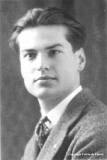
\includegraphics[width=\threefig]{\figdir/deFinetti.jpg}
      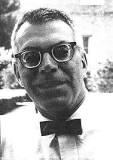
\includegraphics[width=\threefig]{\figdir/savage.jpg}
      \caption{Bruno de Finetti (1906--1985) and L. Jimmie Savage (1917--1971)}
    \end{figure}
  \end{itemize}
\end{frame}

\begin{frame}{Savage's axioms 1/2}
\begin{itemize}
\item Start with the triple $(\cS,\cZ,\cA\subset \cF(\cS, \cZ))$ as in \cite{Wal50}.
\item Savage's idea is to list what we expect from a binary relation $\prec$ on $\cA\times \cA$ describing a decision maker's preferences.
\end{itemize}
\blank
\blank
\end{frame}

\begin{frame}{Savage's axioms 2/2}
\end{frame}

\begin{frame}{De Finetti's theorem (Hewitt-Savage form)}
  \begin{block}{Theorem: exchangeable $\leftrightarrow$ conditionally i.i.d.; see\citep[Theorem 1.49]{Sch95}}
    Let $X_1,X_2,\dots$ be a sequence of exchangeable random variables on $\cX$, i.e.
    $$
    X_1,\dots,X_n \sim X_{\pi(1)},\dots, X_{\pi(n)}, \forall n, \forall \pi\in\frak S_n.
    $$
    Then there exists a probability distribution $\mu$ \un{on the set of probability measures $\mathcal P(\cX)$ on $\cX$} such that
    $$
    \mathbb P (X_1\in A_1, \dots, X_n\in A_n) = \int Q(A_1)\dots Q(A_n)\d\mu(Q).
    $$
    Furthermore, if $Q\sim\mu$,
    $$
    Q(A) = \lim_{n\rightarrow\infty} \frac 1n\sum_{i=1}^n 1_A(X_i).
    $$
  \end{block}
  To a subjectivist, Savage's theorem says you should use SEU, and representation theorems like de Finetti's constrain your choice of $p$.
\end{frame}

\begin{frame}{De Finetti's theorem and LDA}
\end{frame}

\begin{frame}{Bonus: The Dirichlet process through de Finetti's theorem}

\begin{block}{The Blackwell-McQueen urn scheme (aka the CRP)}
  Start with an urn containing a single black ball with weight $\alpha$. Repeat: draw a ball from the urn with probability $\propto$ its weight. Then,
  \begin{itemize}
    \item If the ball is black, return it to the urn along with another ball of weight 1, with a new color sampled from some base measure $H$.
    \item If the ball is colored, return it to the urn along with another ball of weight 1 of the same color.
  \end{itemize}
  Denote by $X_1,\dots$ the color of the ball added.
\end{block}
\vfill
\begin{itemize}
  \item Exercise: show that $X_1,X_2,...$ are exchangeable.
  \item The corresponding prior $\mu$ on $\mathcal{P}(\cX)$ is the Dirichlet process with concentration $\alpha$ and base measure $H$.
\end{itemize}
\end{frame}


\begin{frame}{Flaws in the subjectivist viewpoint}
\end{frame}



% % ###############################################
% \subsection{Logic/positivist Bayesians}
% % ###############################################
% \begin{frame}
%   \frametitle{The logical justification}
%   \begin{itemize}
%     \item Top requirement is to find a version of propositional logic that allows taking into account uncertainty.
%     \item Also favourizes interpreting \un{probability distributions as beliefs}, but aims for objective priors.
%     \begin{figure}
%       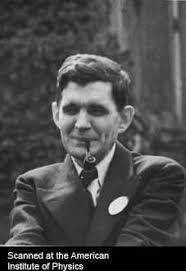
\includegraphics[width=\threefig]{\figdir/cox.jpg}
%       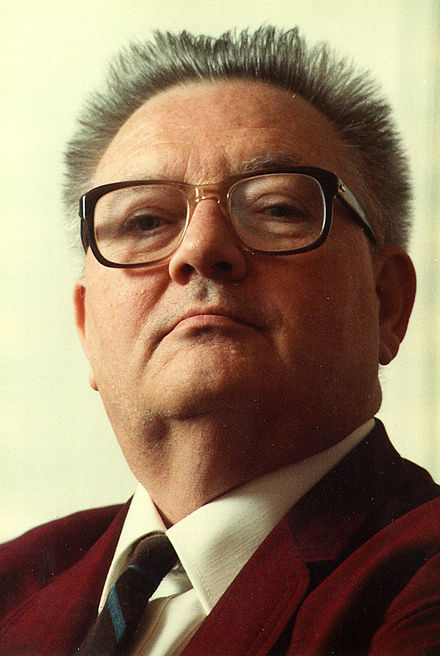
\includegraphics[width=\threefig]{\figdir/jaynes.jpg}
%       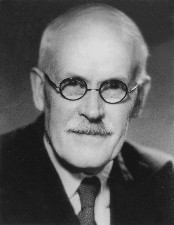
\includegraphics[width=\threefig]{\figdir/jeffreys.jpg}
%       \caption{Richart T. Cox (1898--1991), Edwin T. Jaynes (1917--1971), and Harold Jeffreys (1891--1989)}
%     \end{figure}
%   \end{itemize}
% \end{frame}

% ###############################################
\subsection{Objective Bayes}
\begin{frame}{Objective (or consensual) Bayes}
\begin{itemize}
\item A historical objection to Bayes is the need to choose a prior.
\item By ``objective", we mean that the prior is chosen by some external rule, and that this rule is relatively consensual.
\item Take for instance, Jeffreys's ``noninformative" priors.
\blank
\end{itemize}
\end{frame}
% ###############################################

\subsection{Frequentist Bayes}

\begin{frame}{Complete class theorems state that there is a good prior (but which one?)}

\begin{block}{A complete class theorem for estimation \citep{Ber85}}
Under topological and Euclidean assumptions, if further \begin{itemize}
\item $L(\theta,\cdot)$ is continuous,
\item $\theta\mapsto \int L(\theta,\hat\theta)p(y_{1:n} \vert x_{1:n}, \theta)\d y_{1:n}$ is continuous for any $\hat\theta$,
\end{itemize}
then \un{for any estimator $\tilde\theta$} there exists a prior and a corresponding Bayes estimator
$$
\hat\theta_{\text{Bayes}} \in \argmin_{\hat\theta} \mathbb{E}_{\theta\vert x_{1:n},y_{1:n}} L(\theta,\hat\theta)
$$
such that
$$ \forall \theta, \quad \mathbb E_{y_{1:n}\vert x_{1:n},\theta} L(\theta,\hat\theta_{\text{Bayes}}) < E_{y_{1:n}\vert x_{1:n},\theta} L(\theta,\tilde\theta).$$
\end{block}
\begin{alertblock}{Bayesian estimators thus have good frequentist properties}
But finding the ``right" prior can be difficult. Frequentists typically use Bayesian derivations with particular (often data-dependent) priors; see e.g. empirical Bayes procedures \citep{Efr10}.
\end{alertblock}
\end{frame}

\begin{frame}{PAC-Bayesian learning}
\begin{block}{PAC bounds; see e.g. \citep{ShBe14}}
Let $(x_{1:n},y_{1:n})\sim \mathbb{P}^{\otimes n}$, and independently $(x,y)\sim \mathbb{P}$, we want an algorithm $g(\cdot; x_{1:n}, y_{1:n})\in\mathcal G$ such that if $n\geq n(\delta,\epsilon)$,
$$
\unn{\mathbb{P}^{\otimes n}}\left[\mathbb{E}_{(x,y)\sim \mathbb P} L(a_g,s) \leq \epsilon\right] \geq 1-\delta.
$$
\end{block}
\begin{block}{McAllester's bound for 0-1 loss (Chapter 31 of the above book)}
For any two distributions $P,Q$ on $\mathcal G$, with $\unn{\mathbb{P}^{\otimes n}}$-probability $1-\delta$,
$$
\mathbb E_{g\sim Q} \un{\mathbb{P} (g(x)\neq y)} \leq \mathbb{E}_{g\sim Q} \unnnn{\frac1n\sum_{i=1}^n 1_{g(x_i)\neq y_i}} + \sqrt{\frac{\text{KL}(Q,P) + \log(n/\delta)}{2(n-1)}}.
$$
\end{block}

This suggests taking the ``posterior" $Q$ to be in
$$
\argmin \mathbb{E}_{g\sim Q} \unnnn{\frac1n\sum_{i=1}^n 1_{g(x_i)\neq y_i}} + \sqrt{\frac{\text{KL}(Q,P) + \log(n/\delta)}{2(n-1)}}.
$$
\end{frame}


\subsection{Most people are hybrid Bayesians}
\begin{frame}
  \frametitle{One possible hybrid view, e.g. \citep{Rob07}}
  \begin{itemize}
    \item The starting point is Wald's decision setting, adding integration with respect to a prior.
    \item It is simple, widely applicable, has good frequentist properties.
    \item It satisfies the \un{likelihood principle}.
    \item It is tempting to interpret it as follows: beliefs are
    \begin{itemize}
      \item represented by probabilities,
      \item updated using Bayes' rule,
      \item integrated when making decisions.
    \end{itemize}
    \item It is easy to communicate your uncertainty
    \begin{itemize}
      \item Simply give your posterior.
      \item When making a decision, make sure that the priors of everyone involved would yield the same decision.
      \item Alternately, perform a \un{prior sensitivity analysis}.
    \end{itemize}
  \end{itemize}
\end{frame}

\subsection{Discussion}
\begin{frame}{What kind of Bayesian are you?}
\begin{itemize}
\item I've only scratched the surface. See e.g. \citep{May18}.
\item Posterior expected utility is conceptually simple and unifying. Beyond that, \un{many intepretations get (partial) philosophical support}.
\item The role of the likelihood, the prior, your update mechanism, etc. depend on the intepretation that you choose.
\item[\frownie] \un{Many people do not care}.
\item Hybrid views have become common among statisticians \citep{Rob07,GCSDVR13}, but this arguably makes the role of priors fuzzy.
\item In ML, the development of \un{Bayesian nonparametrics is reviving the subjectivist view}, while objective approaches like \un{PAC-Bayes are also increasingly popular}.
\item A great entry on subjective Bayes is \citep{PaIn09}.
\end{itemize}
\end{frame}

\section{Take-home messages}
\begin{frame}
\end{frame}
  


% From linear regression to GPs
% Example regression
% Bayesian optimization
% Applications to hyperparameter tuning

%\includegraphics[width=.9\textwidth]{salsify}

\section*{References}
\setbeamertemplate{bibliography item}[text]%,
\begin{frame}[allowframebreaks]
\frametitle{References}
\small
\printbibliography
\normalsize
\end{frame}
\end{document}
